\section{Next Generation Deep Learning}

\subsection{Supervised Learning}
Most deep learning follows the supervised paradigm, which is a mapping task learned from input-output pairs.\\

The harder the task the more training data is required.\\

What makes a task hard? \f{\to} Dimensionality and complexity of the data

\subsection{Unsupervised Learning}
Motivation: there are (almost) arbitrary amounts of unlabeled data. Ideally, we could learn from these. This is called unsupervised or self-supervised learning.\\

Self-supervised pretraining is competitive with supervised pretrainingon the ImageNet classification task.\\

Problem: If the output is undefined, the network can learn anything. What is a good training objective?\\

Traditional approach: Reconstruct the output (autoencoder) and compute reconstruction error.\\

\b{(Masked) Autoencoders\\[0.5em]}
Autoencoders typically do not learn semantically meaningful features since the reconstruction loss cares about pixel details, not semantics.\\

\b{Masking} some input image patches forces the encoder to care more about semantics as new content must be generated by the decoder based on the encoded context.\\

\b{Note:} Bottleneck acts as dimensionality reduction.\\

\b{Exemplar CNN\\[0.5em]}
An alternative approach to Masked Autoencoders. Involves training a network to discriminate surrogate classes. Each class is defined by a random seed patch and its transformed versions(translation, rotation, scaling, color, contrast, brightness, blur). This can also be seen as a extreme version of data augmentation. The transformations define invariance properties of the features to be learned.\\

\b{Contrastive Learning\\[0.5em]}
The principle of surrogate classes can be generalized to a contrastive loss to learn a feature embedding. \\

Main idea: for a sample define another positive sample that should be close in embedding space, and multiple negative samples that should be far. Positives and negatives can often be defined without supervision (self-supervised).\\

See DL summary for more!\\
\newpage

\b{DINO\\[0.5em]}
DINO uses a loss similar to a contrastive loss but with only positive samples: maximizing the similarity of the output distribution (cross-entropy).\\

To avoid collapse without negative samples, the teacher is updated only via the exponential moving average of the student network.\\

Transformed versions of an image are created (also) by local cropping operations. Only the teacher sees the global view.\\

\b{Other Self-Supervised Tasks\\[0.5em]}
Jigsaw-Puzzles, temporal order prediction

\subsection{Semi-Supervised Learning}
The goal is to combine the best of both worlds of supervised and unsupervised learning: exploit unlabeled data to require fewer labeled samples.\\

\b{Note:} Semi-supervised learning only works if the process that generates y from x is not independent of p(x).\\

\b{Student-Teacher Training\\[0.5em]}
The student is trained on labeled data while the teacher is the time-accumulated model of student models (EMA). The teacher provides an additional consistency loss on unlabeled data (pseudo-labels).\\

\b{Unsupervised Data Augmentation\\[0.5em]}
Label consistency over transformed inputs is used as an additional loss. This can also be seen as a regularizer.\\

\b{Noisy Student\\[0.5em]}
Train teacher model with labeled data \f{\to} Get pseudo-labels on unlabeled data \f{\to} Train equal or larger student with combined data and noise (augmentations) \f{\to} Make the student the new teacher \f{\to} Repeat the process\\

\b{Segmentation with GAN\\[0.5em]}
A segmentation network acts as the generator. It is trained partially on labeled samples using a regular cross-entropy loss. On unlabeled samples, the discriminator score acts as loss (the discriminator gets the input image and the segmentation as input).\\
Here the GAN learns a conditional distribution (input image as condition).


\subsection{Vision-Language Models}
Idea: Learn joint embedding spaces for vision and language. This provides visual grounding for text models and weak supervision for vision models.\\

If this is done with web-scale datasets, the resulting models are called \b{Foundation Model}. These give rise to a whole new set of applications: Multi-modal retrieval (find images via text, or vice-versa), "zero-shot” classification, open vocabulary detection, text-conditioned image generation.
\newpage

\b{CLIP\\[.5em]}
CLIP makes use of the description which are often added to images on the internet to create a shared embedding space.
\begin{figure}[h!]
    \centering
    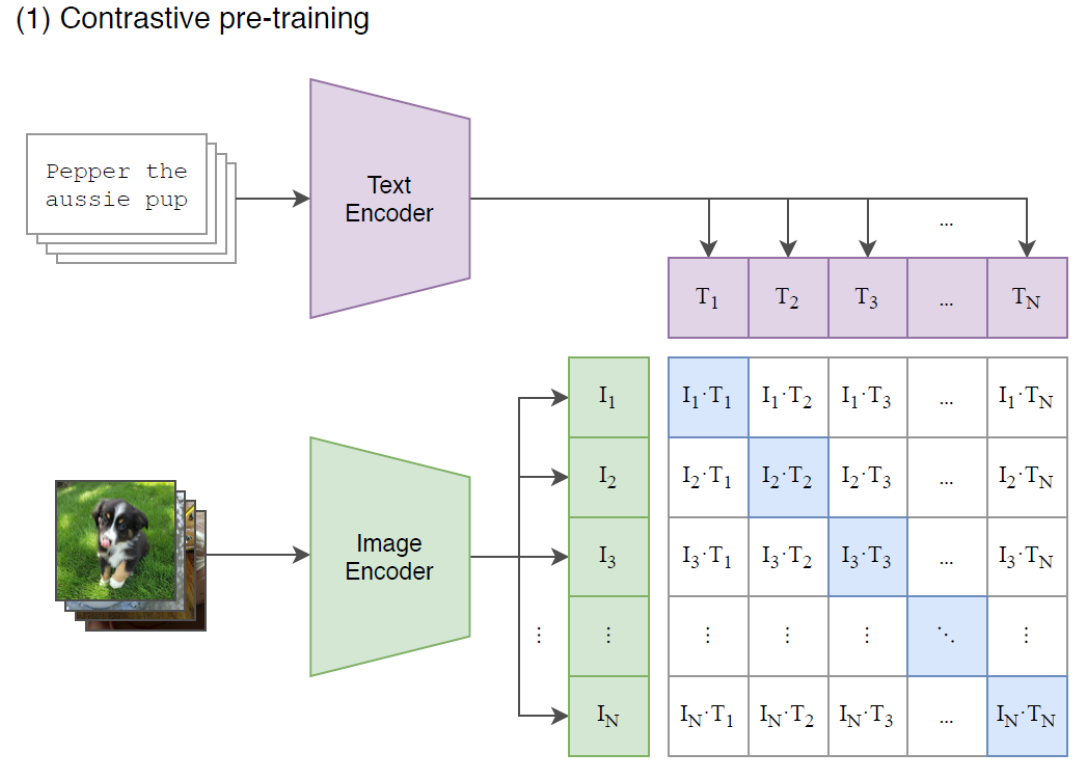
\includegraphics[width=.5\textwidth]{clip.png}
\end{figure}

\b{Distribution Shifts and Foundation Models\\[.5em]}
Most ML learning assumes that the test data is from the same distribution as the training data. Domain gap examples are:
\begin{itemize}
    \item synthetic vs. real data
    \item weather conditions, other backgrounds
    \item new camera with different resolution
\end{itemize}

If a domain gap exists, the source and target domain have to be adapted to fit each other (very tedious). As foundation models cover nearly all domains, they will never be out of distribution. In other words, one can avoid domain adaption by using foundation models (as backbone) for various domains/tasks.\\

To cover all domains, we need very large datasets (web-scale). This amount of data can not be labeled, so foundation models have to rely on self-supervised learning. To produce outputs for a wide variety of data and tasks we need a large model with enough capacity, which makes foundation models extremely compute intensive.\\

\b{Status quo for Foundation Models\\[.5em]}
The currently best working example are Language Models. They leverage the abundance of text available on the internet in combination with a good self-supervised task (next token prediction). The downstream tasks are also very straightforward.\\

Computer Vision is mainly covered by image-language models, as image-language acts as noisy labeling. Note that resource requirements are even larger.